\documentclass{article}
\usepackage{graphicx} 
\usepackage{amsmath}
\usepackage{gauss, amssymb}
\usepackage{nicematrix}
\usepackage[utf8]{inputenc}
\usepackage[T1]{fontenc}
\usepackage[english]{babel}
\usepackage[nottoc,notlot,notlof]{tocbibind}
\usepackage[hidelinks]{hyperref}
\usepackage{amsthm}
\usepackage{physics}
\usepackage{booktabs}
\usepackage{nicematrix}
\usepackage{tikz}

\theoremstyle{definition}
\newtheorem{definition}{Definition}[section]


\newcommand{\mycomment}[1]{}

% Define \circled
\newcommand*\circled[1]{\tikz[baseline=(char.base)]{
            \node[shape=circle,draw,inner sep=1pt] (char) {#1};}}

\title{5705.25 - Hagfrøðilig læring H25}
\date{\today}
%This material is based upon the book 
\begin{document}

\maketitle

\tableofcontents

\newpage

\input{chapters/chapter_01.tex}
\newpage
\section{Statistical Learning}

Statistical learning is concerned with understanding and estimating the relationship between a target variable \( Y \) and one or more predictors \( X = (X_1, X_2, \ldots, X_p) \).  
We typically assume the model:
\[
Y = f(X) + \epsilon
\]
where \( f(X) \) is the systematic part of the relationship, and \( \epsilon \) is random noise with mean zero.

\subsection{Supervised Learning}

In supervised learning, both the predictors \( X \) and the response \( Y \) are observed, and the goal is to estimate the mapping \( f: X \mapsto Y \).

\subsubsection{Types of Supervised Learning}
Depending on the type of \( Y \), we distinguish between:

\begin{center}
\begin{tabular}{@{}lll@{}}
\toprule
Type of \( Y \) & Task & Example \\
\midrule
Continuous (quantitative) & Regression & Predicting sales, temperature, price \\
Discrete (qualitative) & Classification & Predicting spam vs.\ non-spam, disease vs.\ healthy \\
\bottomrule
\end{tabular}
\end{center}

\subsubsection{Example: Predicting Sales}
Suppose we want to predict sales \( Y \) using advertising budgets in three media channels:
\[
X_1 = \text{TV}, \quad X_2 = \text{Radio}, \quad X_3 = \text{Newspaper.}
\]
We assume
\[
Y = f(X_1, X_2, X_3) + \epsilon
\]
and start with a linear model:
\[
f(X) = \beta_0 + \beta_1 X_1 + \beta_2 X_2 + \beta_3 X_3.
\]

\subsubsection{Estimating \( f \) Using Squared Loss}

To estimate \( f \), we minimize the squared loss:
\[
L(y_i, \hat{f}(x_i)) = (y_i - \hat{f}(x_i))^2,
\]
and the total (mean) squared error:
\[
\text{MSE}(\hat{f}) = \frac{1}{n}\sum_{i=1}^{n}(y_i - \hat{f}(x_i))^2.
\]

The optimal parameters \( \beta_j \) are found by minimizing the MSE, leading to the ordinary least squares (OLS) solution:
\[
\hat{\boldsymbol{\beta}} = (X^T X)^{-1} X^T y.
\]

\subsection{Unsupervised Learning}

In unsupervised learning, only the predictors \( X \) are observed; there is no corresponding response variable \( Y \).  
The goal is to discover structure or patterns within the data.

\subsubsection{Clustering}
A common example is \textbf{clustering}, where observations are grouped based on similarity among predictors \( X_1, X_2, \ldots \).  
For instance, clustering points \( (x_1, x_2) \) may reveal natural groupings or clusters within a dataset.

\subsubsection{Outcomes}
In contrast to supervised learning:
\begin{itemize}
    \item Continuous outcomes correspond to \textbf{regression}.
    \item Discrete outcomes correspond to \textbf{classification}.
\end{itemize}

\subsection{Least Squares Regression}

In least squares regression, we assume a model such as:
\[
f(X) = \beta_0 + \beta_1 X_1 + \beta_2 X_1^2,
\]
which can capture some curvature or nonlinearity.

While more flexible models can better fit training data, they also introduce new issues such as \textbf{overfitting}.  
We can measure performance using the Mean Squared Error (MSE):
\[
\text{MSE} = \frac{1}{n}\sum_{i=1}^{n} (y_i - \hat{f}(x_i))^2.
\]

The error can be decomposed into:
\begin{itemize}
    \item \textbf{Training error}: computed on the same data used to fit the model.
    \item \textbf{Test (validation) error}: computed on unseen data.
\end{itemize}

A model that fits the training data too closely may not generalize well to new data this is overfitting.  
The aim is to find a balance between underfitting and overfitting.

As a general rule of thumb, more flexible methods tend to perform better than inflexible ones, but they must be validated using separate \textbf{validation} and \textbf{test} sets.

\subsection{Bias--Variance Tradeoff}

The expected prediction error for a given \( x_0 \) can be decomposed as:
\[
\mathbb{E}\big[(Y - \hat{f}(x_0))^2\big] = 
\big[\text{Bias}(\hat{f}(x_0))\big]^2 + \text{Var}(\hat{f}(x_0)) + \sigma_\epsilon^2,
\]
where:
\begin{itemize}
    \item \( \sigma_\epsilon^2 = \text{Var}(\epsilon) \) is the irreducible error,
    \item \( \text{Bias}(\hat{f}(x_0)) = \mathbb{E}[\hat{f}(x_0)] - f(x_0) \),
    \item \( \text{Var}(\hat{f}(x_0)) \) is the variability of the estimate.
\end{itemize}

We cannot reduce the irreducible error, but we can trade off bias and variance.  
Accuracy depends on finding the right balance:
\begin{itemize}
    \item High bias \(\Rightarrow\) underfitting.
    \item High variance \(\Rightarrow\) overfitting.
\end{itemize}

Interpretability often decreases as model flexibility increases.

\subsection{Classification}

In classification, the goal is to predict a qualitative response \( Y \) taking values in a finite set of classes \( \{1, 2, \ldots, K\} \).

\subsubsection{K-Nearest Neighbours (KNN)}
Given a new observation \( x_0 \), KNN identifies the \( K \) training points closest to \( x_0 \) (denoted \( \mathcal{N}_0 \)) and estimates:
\[
\Pr(Y = j \mid X = x_0) = \frac{1}{K} \sum_{i \in \mathcal{N}_0} I(Y_i = j),
\]
where \( I(\cdot) \) is the indicator function.

The predicted class is:
\[
\hat{y}_0 = \arg\max_j \Pr(Y = j \mid X = x_0).
\]

\subsubsection{Classification Error}
The classification error rate is:
\[
\text{Error} = \frac{1}{K} \sum_{i \in \mathcal{N}_0} I(Y_i \neq \hat{Y}_i).
\]

\subsubsection{Bayes Classifier}
The Bayes classifier assigns each observation to the most probable class:
\[
\hat{y}_{\text{Bayes}} = \arg\max_j \Pr(Y = j \mid X = x),
\]
which theoretically minimizes the classification error.  
In practice, methods like KNN approximate this boundary, sometimes sacrificing perfect classification to reduce noise.

\subsubsection{Key Idea}
A fundamental rule to remember is:
\[
Y = f(X) + \epsilon.
\]
This holds true for both regression and classification settings the goal of statistical learning is to estimate \( f \) as accurately as possible.

 

\newpage
\section{Regression}

Regression analysis is a fundamental statistical technique used to model and understand the relationship between a response variable \( Y \) and one or more explanatory variables \( X_1, X_2, \ldots, X_p \). The goal is to estimate a function \( f(X) \) that captures the systematic relationship between \( X \) and \( Y \), while accounting for random variation (error).

\subsection{Additive Error Models}

We often assume an additive model of the form:
\[
Y = f(X) + \varepsilon,
\]
where \( \varepsilon \) is a random error term with
\[
\mathbb{E}[\varepsilon] = 0, \quad \text{and} \quad \text{Var}(\varepsilon) = \sigma^2.
\]
The term \( \varepsilon \) captures the \textbf{irreducible error}—random variation that cannot be explained by the model, even with perfect knowledge of \( f \).

A common goal is to estimate the \textbf{regression function}:
\[
f(X) = \mathbb{E}[Y|X].
\]
This represents the expected value of \( Y \) for a given value of \( X \).

\subsection{Estimating \( f(X) \)}

Given a set of training data \((x_1, y_1), \ldots, (x_n, y_n)\), we want to construct an estimate \(\hat{f}(X)\) that minimizes the expected prediction error:
\[
\mathbb{E}\left[(Y - \hat{f}(X))^2\right].
\]

\subsubsection{K-Nearest Neighbour (KNN) Regression}

A simple non-parametric estimator is the \textbf{K-nearest neighbours (KNN)} regression:
\[
\hat{f}(x_0) = \frac{1}{K} \sum_{x_i \in \mathcal{N}_K(x_0)} y_i,
\]
where \(\mathcal{N}_K(x_0)\) is the set of the \(K\) closest training points to \(x_0\).

\paragraph{Example:}
For example, to predict \( f(4) \), we take the average of the \(Y_i\) values for the \(K\) data points whose \(X_i\) values are closest to \(4\):
\[
\hat{f}(4) = \text{avg}\{Y_i : X_i \in \mathcal{N}_K(4)\}.
\]

\paragraph{Advantages and Limitations:}
\begin{itemize}
    \item Performs well when the number of predictors \(p\) is small and sample size \(n\) is large.
    \item Performs poorly when \(p\) is large due to the \textbf{curse of dimensionality}—as \(p\) increases, points become sparse, and distances between them lose meaning.
\end{itemize}

\begin{center}
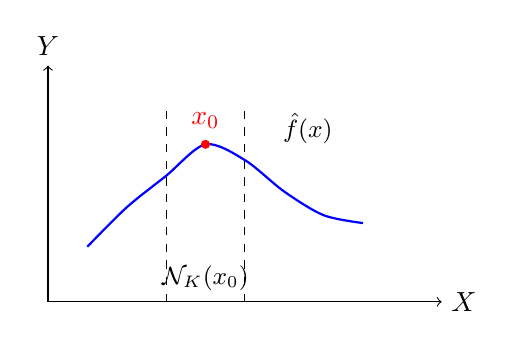
\begin{tikzpicture}[scale=1.0]
\draw[->] (0,0) -- (5,0) node[right] {$X$};
\draw[->] (0,0) -- (0,3) node[above] {$Y$};
\draw[blue, thick] plot[smooth] coordinates {(0.5,0.7) (1,1.2) (1.5,1.6) (2,2) (2.5,1.8) (3,1.4) (3.5,1.1) (4,1)};
\node at (3.3,2.2) {\small $\hat{f}(x)$};
\draw[red, fill=red] (2,2) circle (0.05);
\node[red] at (2,2.3) {$x_0$};
\draw[dashed] (1.5,0) -- (1.5,2.5);
\draw[dashed] (2.5,0) -- (2.5,2.5);
\node at (2,0.3) {\small $\mathcal{N}_K(x_0)$};
\end{tikzpicture}

\textit{Figure: KNN regression—averaging points within a neighbourhood around \(x_0\).}
\end{center}

\subsection{Parametric Models and Linear Regression}

To overcome the limitations of non-parametric methods like KNN, we often use a \textbf{parametric model} that assumes a specific functional form for \( f(X) \):
\[
f(X) = \beta_0 + \beta_1 X_1 + \beta_2 X_2 + \dots + \beta_p X_p.
\]

Even though this form is rarely exactly true, it provides a simple and interpretable approximation.

\subsubsection{Simple Linear Regression}

For a single predictor variable:
\[
Y = \beta_0 + \beta_1 X + \varepsilon.
\]

The goal is to estimate \( \beta_0 \) and \( \beta_1 \) using the training data, such that the \textbf{residual sum of squares (RSS)} is minimized:
\[
\text{RSS} = \sum_{i=1}^{n} (y_i - \hat{y}_i)^2 = \sum_{i=1}^{n} (y_i - \hat{\beta}_0 - \hat{\beta}_1 x_i)^2.
\]

Setting the partial derivatives of RSS with respect to \(\beta_0\) and \(\beta_1\) equal to zero yields the least-squares estimates.

\paragraph{Population Regression Line Example:}
\[
Y = 2 + 3X + \varepsilon \quad \Rightarrow \quad f(X) = 2 + 3X.
\]
Here, \(\beta_0 = 2\) and \(\beta_1 = 3\) are unbiased estimates of the true relationship between \(X\) and \(Y\).

\subsubsection{Standard Errors and Confidence Intervals}

The variance of the error term is denoted \(\sigma^2 = \text{Var}(\varepsilon)\).  
The estimated variance from data is:
\[
\widehat{\sigma}^2 = \frac{\text{RSS}}{n - 2}.
\]

The \textbf{standard error} of \(\hat{\beta}_1\) measures the uncertainty of the slope estimate.

A 95\% confidence interval for \(\beta_1\) is:
\[
[\hat{\beta}_1 - 2 \cdot SE(\hat{\beta}_1), \; \hat{\beta}_1 + 2 \cdot SE(\hat{\beta}_1)].
\]

\subsection{Hypothesis Testing}

We often test whether there is a significant relationship between \(X\) and \(Y\).

\[
\begin{aligned}
H_0 &: \beta_1 = 0 \quad \text{(no relationship)} \\
H_a &: \beta_1 \neq 0 \quad \text{(some relationship)}
\end{aligned}
\]

The test statistic is:
\[
t = \frac{\hat{\beta}_1 - 0}{SE(\hat{\beta}_1)},
\]
which follows a \(t\)-distribution with \(n - 2\) degrees of freedom under \(H_0\).

The \textbf{p-value} is the probability of observing a \( |t| \) as large as the one obtained, assuming \(H_0\) is true.  
A small p-value (typically \(< 0.05\)) leads to rejection of \(H_0\).

\subsection{Assessing Model Accuracy}

\subsubsection{Residual Standard Error (RSE)}

The RSE provides an estimate of the standard deviation of the residuals:
\[
RSE = \sqrt{\frac{RSS}{n - 2}}.
\]

\subsubsection{The \(R^2\) Statistic}

The \(R^2\) statistic measures the proportion of variability in \(Y\) explained by the model:
\[
R^2 = 1 - \frac{RSS}{TSS},
\]
where
\[
TSS = \sum_{i=1}^{n} (y_i - \bar{y})^2.
\]
Here, \(TSS\) measures the total variance in \(Y\), and \(RSS\) measures the remaining variability after regression.

\paragraph{Properties:}
\begin{itemize}
    \item \(R^2\) typically lies between 0 and 1.
    \item It can be negative for models that fit worse than a horizontal line at \(\bar{y}\).
    \item \(R^2\) is independent of the units of \(Y\).
\end{itemize}

\subsection{Bias–Variance Tradeoff}

When fitting regression models, we balance two sources of error:
\[
\text{Expected Test Error} = \text{Bias}^2 + \text{Variance} + \text{Irreducible Error}.
\]
Parametric models typically have higher bias but lower variance, while non-parametric models like KNN have lower bias but higher variance.

\subsection{Software Note: R and Quarto}

When working with R in VSCode, you can compile regression analyses and visualizations within \texttt{.qmd} (Quarto) files, which support both code and markdown text for reproducible reports.


\newpage
\section{Classification}

Classification problems involve predicting a qualitative (categorical) response variable \(Y\) based on one or more predictor variables \(X\).  

\subsection{Quantitative vs. Qualitative Outcomes}

\begin{itemize}
    \item \textbf{Quantitative outcomes:} \(Y \in \mathbb{R}\). Typically modeled with regression, minimizing a loss function such as least squares.
    \item \textbf{Qualitative outcomes:} \(Y \in \{1, 2, \dots, K\}\). These are modeled using classification methods like logistic regression or generative models.
\end{itemize}

\subsection{Feature Vector and Notation}

Let 
\[
\mathbf{X} = (X_1, X_2, \dots, X_p)^T
\] 
be the feature vector. For example, in the \textbf{IRIS dataset}, the features are:
\[
X_1 = \text{Sepal Length}, \quad X_2 = \text{Sepal Width}, \quad X_3 = \text{Petal Length}, \quad X_4 = \text{Petal Width}
\] 
and the response \(Y \in \{\text{setosa, versicolor, virginica}\}\).

The predicted class is:
\[
g(\mathbf{x}) = \arg\max_{k} P(Y = k \mid \mathbf{X} = \mathbf{x})
\]

\subsection{Logistic Regression (Binary Case)}

The probability of class 1 is modeled as:
\[
P(Y=1 \mid X=x) = \frac{e^{\beta_0 + \beta_1 x}}{1 + e^{\beta_0 + \beta_1 x}}
\]

The log-odds (logit) transformation gives a linear relationship:
\[
\log \frac{P(x)}{1 - P(x)} = \beta_0 + \beta_1 x
\]

\[
\begin{cases} 
\beta_1 > 0 & \text{increasing $x$ increases $P(x)$} \\
\beta_1 < 0 & \text{increasing $x$ decreases $P(x)$} 
\end{cases}
\]

\subsection{Maximum Likelihood Estimation (MLE)}

The likelihood function is:
\[
L(\beta_0, \beta_1) = \prod_{i=1}^{n} P(x_i)^{y_i} \left[ 1 - P(x_i) \right]^{1 - y_i}
\]

MLE maximizes the likelihood (or equivalently, minimizes the negative log-likelihood):
\[
\hat{\beta}_0, \hat{\beta}_1 = \arg\max_{\beta_0, \beta_1} L(\beta_0, \beta_1)
\]

\subsection{Multinomial Logistic Regression}

For \(K>2\) classes, probabilities are modeled using the \textbf{softmax function}:
\[
P(Y=k \mid X=x) = \frac{e^{\beta_{k0} + \beta_k^T x}}{\sum_{j=1}^{K} e^{\beta_{j0} + \beta_j^T x}}
\]

The log-odds relative to a baseline class \(K\) are:
\[
\log \frac{P(Y=k \mid X=x)}{P(Y=K \mid X=x)} = \beta_{k0} + \beta_k^T x
\]

\subsection{Generative Models}

Generative models estimate:
\[
P(X \mid Y=k) \quad \text{and} \quad P(Y=k)
\] 
Then, using Bayes' theorem:
\[
P(Y=k \mid X=x) = \frac{P(X=x \mid Y=k) P(Y=k)}{\sum_{j=1}^K P(X=x \mid Y=j) P(Y=j)}
\]

\subsection{Additive Models and Least Squares}

For continuous responses:
\[
Y = f_\theta(X) + \epsilon, \quad \epsilon \sim N(0, \sigma^2)
\]

MLE reduces to minimizing the sum of squared errors (RSS):
\[
\hat{\theta} = \arg\min_\theta \sum_i \left( Y_i - f_\theta(X_i) \right)^2
\]

\subsection{Visualizing Logistic Regression Decision Boundary}

\begin{tikzpicture}[scale=1.0]
\draw[->] (0,0) -- (6,0) node[right] {$X$};
\draw[->] (0,0) -- (0,4) node[above] {$P(Y=1|X)$};
\draw[domain=0:5, smooth, variable=\x, blue, thick] plot ({\x}, {4/(1+exp(-1*(\x-2)))});
\draw[dashed] (2,0) -- (2,2) -- (0,2);
\node at (3.5,3.5) {Sigmoid curve};
\node at (2.5,0.3) {$x_0$};
\end{tikzpicture}

\subsection{Generative Models and Advanced Classification}

Generative models estimate the joint distribution \(P(X,Y)\) and then use Bayes' theorem to compute class probabilities:
\[
P(Y=k \mid X=x) = \frac{P(Y=k) P(X=x \mid Y=k)}{P(X=x)}
\]

Here:
\begin{itemize}
    \item \(P(Y=k)\) is the prior probability of class \(k\)
    \item \(P(X=x \mid Y=k)\) is the class-conditional density
    \item \(P(X=x) = \sum_{i=1}^K P(Y=i) P(X=x \mid Y=i)\) by the law of total probability
\end{itemize}

\subsubsection{Linear Discriminant Analysis (LDA)}

LDA assumes that:
\begin{itemize}
    \item Each class \(k\) has a Gaussian distribution with mean \(\mu_k\) and a **common covariance matrix** \(\Sigma\)
    \item The decision boundary is linear in \(x\)
\end{itemize}

The discriminant function is:
\[
\delta_k(x) = x^T \Sigma^{-1} \mu_k - \frac{1}{2} \mu_k^T \Sigma^{-1} \mu_k + \log \pi_k
\]
where \(\pi_k\) is the prior probability of class \(k\).  

The predicted class is:
\[
\hat{y} = \arg\max_k \delta_k(x)
\]

We estimate unknown parameters from the data:
\[
\hat{\mu}_k = \frac{1}{n_k} \sum_{i: y_i=k} x_i, \quad
\hat{\Sigma} = \frac{1}{n-K} \sum_{k=1}^K \sum_{i: y_i=k} (x_i - \hat{\mu}_k)(x_i - \hat{\mu}_k)^T
\]

\subsubsection*{Decision Boundary Visualization (2 Classes, 2 Features)}
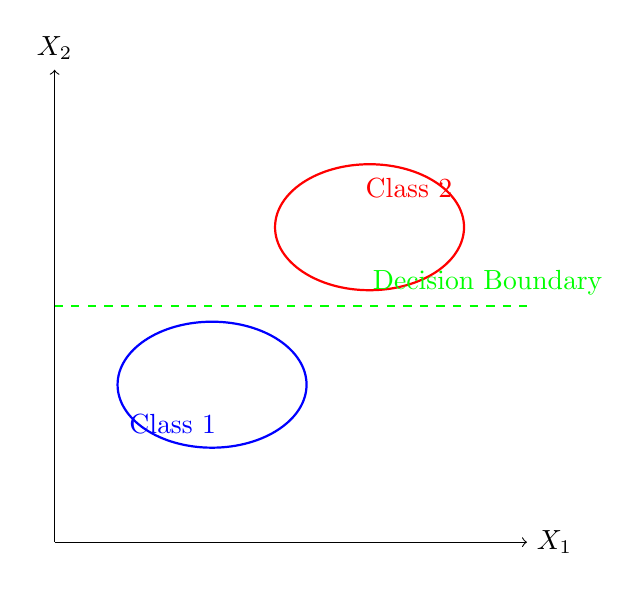
\begin{tikzpicture}[scale=1.0]
% axes
\draw[->] (0,0) -- (6,0) node[right] {$X_1$};
\draw[->] (0,0) -- (0,6) node[above] {$X_2$};

% class 1 ellipse
\draw[blue, thick] (2,2) ellipse (1.2cm and 0.8cm);
\node[blue] at (1.5,1.5) {Class 1};

% class 2 ellipse
\draw[red, thick] (4,4) ellipse (1.2cm and 0.8cm);
\node[red] at (4.5,4.5) {Class 2};

% linear decision boundary
\draw[green, thick, dashed] (0,3) -- (6,3);
\node[green] at (5.5,3.3) {Decision Boundary};
\end{tikzpicture}

\subsubsection{Quadratic Discriminant Analysis (QDA)}

QDA relaxes the LDA assumption of common covariance matrices:
\[
\Sigma_k \neq \Sigma_j \quad \text{for some } k \neq j
\]

The discriminant function becomes quadratic:
\[
\delta_k(x) = -\frac{1}{2} \log |\Sigma_k| - \frac{1}{2} (x - \mu_k)^T \Sigma_k^{-1} (x - \mu_k) + \log \pi_k
\]

\subsubsection{Naive Bayes Classifier}

Naive Bayes assumes that features are conditionally independent given the class:
\[
P(X_1, X_2, \dots, X_p \mid Y=k) = \prod_{j=1}^p P(X_j \mid Y=k)
\]

This allows simple estimation using Gaussian distributions for quantitative features or categorical probabilities for discrete features.

\subsubsection{K-Nearest Neighbors (KNN)}

\begin{itemize}
    \item Non-parametric and flexible
    \item Assigns a class based on the majority vote of the \(K\) nearest neighbors in feature space
    \item More data generally improves performance
\end{itemize}

\subsubsection{Bias-Variance Trade-off and Model Comparison}

\begin{itemize}
    \item LDA: Linear boundaries, low variance, higher bias
    \item QDA: Quadratic boundaries, higher variance, lower bias
    \item Logistic Regression: Linear boundary, sensitive to collinearity
    \item KNN: Highly flexible, low bias, potentially high variance
\end{itemize}

\subsubsection{Performance Metrics}

\begin{itemize}
    \item \textbf{Accuracy:} Overall correct classification
    \item \textbf{Sensitivity / Recall:} True positive rate
    \item \textbf{Specificity:} True negative rate
    \item \textbf{ROC curve:} Trade-off between sensitivity and false positive rate
\end{itemize}

\subsubsection{Other Notes}

\begin{itemize}
    \item Poisson regression for count data: \(n \sim \text{Poisson}(\mu)\) with \(\log(\mu) = X \beta\)
    \item More data allows more flexible models (e.g., QDA, KNN) to perform well without overfitting
\end{itemize}


\end{document}
